
\chapter{Estado da arte}
%Para a organização do trabalho foi utilizada a técnica de desenvolvimento ágil SCRUM
De forma a organizar todo o trabalho a desenvolver visto que este é dividido com mais uma colega, 
foi então utilizada a técnica de desenvolvimento ágil, conseguindo assim organizar todas as tarefas 
entre os elementos de desenvolvimento do projeto.

\section{Ferramentas de trabalho utilizadas}

A organização de todas as tarefas, foi realizada na ferramenta \textit{Github Projetcs}, esta 
permite ligar um projeto a um repositório de \textit{Github}, conseguindo também personalizar completamente todo 
o projeto e parâmetros das tarefas o que permite uma organização minuciosa destas.

O Microsoft Excel foi também utilizado para a engenharia de \textit{software} onde foram descritos os requisitos 
do projeto, \textit{user stories} e também a especificação de casos de uso. Esta ferramenta foi também utilizada 
para a organização de reuniões com o cliente e redação de tópicos a abordar e abordados nesta.

Para o desenvolvimento do \textit{design do software} foi utilizado a ferramenta \textit{figma}, que permite o \textit{design} de 
todas as componentes tendo em conta as reais dimensões de um dispositivo. Esta ferramenta 
permite também criar uma apresentação interativa que consegue demonstrar o comportamento da aplicação 
como completamente desenvolvida, dando também suporte à implementação.

O \textit{draw.io} foi também utilizado para o desenho das arquiteturas do projeto tendo se revelado de grande auxílio 
visto que este permite uma grande liberdade no desenho. Esta ferramenta permite também 
conexão com \textit{github} conseguindo assim facilmente guardar estes projetos e ter acesso a partir de qualquer 
dispositivo.

A engenharia de \textit{software} foi realizada através da utilização \textit{Visual Studio paradigm}, esta é uma ferramenta muito 
completa contendo modelos e regras para a engenharia de \textit{software}. Esta ferramenta tornou-se um grande 
auxílio no desenvolvimento da base de dados, pois é possível desenhar o modelo e exportar para um ficheiro 
de criação de base de dados.

\newpage

\section{Tecnologias utilizadas}

\subsection{Serviços Backend}

Para a realização da integração entre a aplicação \emph{frontend} e os dados, foi necessário desenvolver uma API para dar suporte a todos os serviços necessários para a aplicação.
API sigla para "\emph{Application Programming Interface} \emph{exposes a set of data and functions to facilitate interactions between computer programs and allow them to exchange information.}" ~\citep{rest_cookbook}.
Estas ferramentas apesar de serem "\emph{designed  to  work  with  other  programs,  they’re  mostly intended to be understood and used by humans writing those other programs}"\citep{api_design}".

\newpage

\subsubsection{Serviços RestFull e SOAP}
Os seviços RestFull "\emph{expose data as resources  and  use  standard  HTTP  methods  to  represent  Create,  Read,Update,  and  Delete  (CRUD)  transactions  against  these  resources}
\citep{api_design}", sendo que a resposta é no formato JSON "\emph{due  to  its  simplicity  and  ease  of  use  with  JavaScript,  JSON  has become the standard for modern APIs}"\citep{api_design}.

Já SOAP é "\emph{nothing  more  than  a  simple  XML-based  envelope  for  the  information  being  transferred,  and  a  set  of  rules  for  translating  application and platform-specific data types into XML representations}"\citep{Snell2002} sendo que a resposta é realizada em XML leva a que "\emph{It relies heavily on XML  standards  like  XML  Schema  and  XML  Namespaces  for  its  definition  and  function}"\citep{Snell2002}. A utilização de XML permite que "\emph{two  applications,  regardless  of  operating  system,  programming  language,  or  any  other  technical  implementation  detail,  may  openly  share  information  using  nothing  more  than  a  simple  message  encoded  in  a  way  that  both  applications  understand}"\citep{Snell2002}.

Por fim foi decidido utilizar Rest devido a ser \emph{much lighter compared to SOAP. It does not require formats like headers to be included in the message, like it is required in SOAP architecture}". Outra maior valia é que "\emph{ it parses JSON, a human readable language designed to allow data exchange and making it easier to parse and use by the computer. It is estimated to be at around one hundred times faster than XML}"\citep{Halili2018}.

\subsubsection{NodeJS}

Para o desenvolvimento do projeto backend foi escolhido \textit{NodeJS}, este surgiu quando "\emph{the original developers took JavaScript, something you could usually only run inside the browser, and they let it run on your machine as a standalone process}"\citep{design_node} isto significa que "\emph{applications using JavaScript outside the context of the browser}"\citep{design_node} .

Para correr \textit{JavaScript} a nível de servidor web e a nível de computador pessoal é utilizado o mesmo motor, "\emph{it's called the V8 JavaScript runtime engine}"\citep{design_node} , este é "\emph{it's an opensource engine that takes JavaScript code and compiles it into much faster machine code.And that's a big part of what makes Node.js so fast}"\citep{design_node} .

\textit{NodeJs} permite a utilização de bibliotecas externas "\emph{by providing the Node Package Manager}"\citep{design_node} , este permite ao desenvolvedor "\emph{to easily install, manage, and even provide  your own modules for a rapidly grown and well-maintained open source repository}"\citep{design_node} .

\textit{NodeJS} foi escolhido para o desenvolvimento \textit{backend}, uma vez que, permite a utilização de \textit{Typescript} para desenvolvimento e por ser vastamente utilizado, o que permite acesso a diversas fontes de informação para resolução de problemas, assim como auxílio ao desenvolvimento.

\newpage

\subsubsection{Typescript}
O typescript "\emph{is  a  bit  unusual  as  a  language  in  that  it  neither  runs  in  an  interpreter  (asPython  and  Ruby  do)  nor  compiles  down  to  a  lower-level  language  (as  Java  and  Cdo).}"\citep{typescript} isto porque este "\emph{compiles  to  another  high-level  language,  JavaScript.}"\citep{typescript}, isto faz com que o Typescript seja visto como "\emph{a  superset  of  JavaScript  in  a  syntactic  sense}"\citep{typescript}.

Todos os programas JavaScript" \emph{are  TypeScript  programs,  but  the  converse  is  not  true... This  is  because  TypeScript adds additional syntax for specifying types}". O sistema de tipagens do TypeScript tem como objetivo "\emph{to  detect  code  that  will  throw  anexception  at  runtime,  without  having  to  run  your  code. ... The  type  checker  cannot always spot code that will throw exceptions, but it will try}"\citep{typescript}.

Esta linguagem de programação foi escolhida para o \textit{backend} devido à capacidade de assegurar as tipagens, o que leva a um maior nível de segurança em termos de lidar com dados recebidos, assim como também a agilização do processo de programação devido à capacidade de prever a maioria dos erros de código.

\subsection{PostgreSQL}
\emph{PostgreSQL} "is an open source object relational database management system"\citep{Juba2015}. Esta "emphasizes extensibility"\citep{Juba2015} o que permite a utilização de extensões desenvolvidas pela comunidade para novas funcionalidades, mas "Also, there are several extensions to access, manage, and monitor PostgreSQL clusters, such as pgAdmin III"\citep{Juba2015}. Esta ferramenta é de aprendizagem simples devido ao facto de "it complies with ANSI SQL standards"\citep{Juba2015}, o que leva a que, qualquer individuo com conhecimentos prévios em \emph{SQL} consiga facilmente aprender esta tecnologia.

\emph{PostgreSQL} foi escolhido visto que a empresa já utiliza vastamente esta tecnologia, mas também porque que é \emph{open source} e não existirem custos associados para este tipo de utilização. A funcionalidade de extensões do mesmo foi utilizada para implementar \emph{id's} que utilizam a estrutura \emph{uuid} para assim dificultar o ataque aos dados visto que é difícil de prever os valores de \emph{id's} dos dados.

\subsubsection{Logging}
Logging é um processo que permite guardar informação(logs) sobre um evento. Neste contexto logging poderá ser utilizado para realizar a monitorização de pedidos e erros. Estas informações poderão até auxiliar na toma de decisões sobre o software e em quais funcionalidades deste software colocar mais atenção.

\subsubsection{Morgan}

Morgan é uma ferramenta que permite extrair dados de um pedido, assim como também a criação de logs, este atua como um middleware do servidor, recebendo qual o tipo de log a ser escrito, sendo estes tipos definidos pela ferramenta. Os principais dados obtidos pela ferramenta são a data e hora do pedido, o tipo de pedido, o serviço pedido, os dados recebidos, a resposta devolvida e também a descrição do sistema utilizado para realizar o pedido. Com estes dados é possível saber que plataforma é mais utilizada no software, quais as horas de maior utilização e quais os serviços mais executados, estes dados permitem direcionar mais recursos para uma indicada plataforma e/ou serviço, assim como também escolher os melhores horários de manutenção dos servidores.

\subsubsection{Gestão de \textit{emails}}\label{sec:emails_send}
O envio de \textit{emails} para os utilizadores, foi desenvolvido através da biblioteca \textit{Nodemailer}, que permite a utilização de um servidor de \textit{SMTP}. Esta ferramenta foi escolhida devido a ser uma das mais utilizadas para este tipo de necessidade, o que permite que exista mais informação sobre a mesma que auxilia a resolução e identificação de erros. 

Para desenvolver o conteúdo dos \textit{emails} foi utilizada a ferramenta \textit{Tabular Email}, esta permite realizar o \textit{design} do conteúdo de um \textit{email}, sendo possível exportar para \textit{html}. A maior dificuldade desta ferramenta é que não permite a utilização de acentuação, e visto que o \textit{html} é gerado por uma máquina este torna-se complicado de navegar e traduzir.

\subsubsection{Agendamento de tarefas}

Um requisito deste projeto foi o envio diário de \textit{emails} com o relatório de notificações ao final do dia. Primeiramente, para realizar o agendamento de tarefas, foi feita uma análise das ferramentas existentes para a realização deste tipo de ações. Deste modo, foram encontradas o \textit{cronetab} e o \textit{node-cron}. A grande diferença entre estas duas ferramentas é que o \textit{cronetab} funciona a nível de servidor, sendo que, o funcionamento tem por base "\emph{run this command at this time
on this date}"\citep{crontab}, este comando poderá por exemplo executar um código para enviar \textit{emails}. Já o \textit{node-cron} trata-se de uma biblioteca de \textit{NodeJs} "\emph{in pure JavaScript for node.js based on GNU crontab}"\citep{node_cron}, este permite o fácil agendamento de tarefas de forma programática, assim como a indicação do código a ser executado sem necessidade de criar comandos.

A hora de execução do código de envio de \textit{emails} poderá variar e necessitar de reprogramação, pelo que, foi optada a utilização do \textit{node-cron}, uma vez que, facilita a utilização e agilizando o processo de reprogramação de horas de envio do relatório de notificações.

\input{sections/chap2/tecnologias_utilizadas/backend/5.segurança.tex}

\subsubsection{Firebase}
Firebase é uma solução que foi comprada pela \textit{Google} em 2014. O seu objetivo é "\emph{to provide the tools and infrastructure that you need to build great apps}"\citep{Moroney2017}, esta alcança este objetivo através da oferta de serviços pré configurados, sendo que "\emph{many of the technologies are available at no cost}"\citep{Moroney2017}.

\textit{Firestorage} também conhecida como \textit{cloud storage}, é um serviço que dispõe "\emph{a simple API that is backed up by Google Cloud Storage}"\citep{Moroney2017}, que permite guardar e transmitir até 1\textit{GB} de ficheiros de forma gratuita.

\textit{Cloud messaging} é também um serviço do \textit{Firebase} que permite "\emph{to reliably deliver messages at no cost}"\citep{Moroney2017}. Este garante que" \emph{Over 98\% of connected devices receive these messages in less than 500ms}"\citep{Moroney2017}. \textit{Cloud messaging} permite a utilização de diversas formas de envio de notificações como "\emph{driven by analytics to pick audiences, or using topics or other methods}"\citep{Moroney2017}.

\textit{Dynamic links} é um serviço do \textit{Firebase} que permite a criação de "\emph{links to an app that contain context about what you want the end user to see in the app}"\citep{Moroney2017}.

Esta ferramenta foi escolhida devido à sua capacidade de fornecer serviços pré configurados de forma gratuita, o que evita o gasto monetário e a alocação de tempo para a configuração de servidores durante o desenvolvimento.

\subsection{Axios}

Para ser possível realizar pedidos a outros serviços externos como \textit{Firebase}, é necessário utilizar uma biblioteca capaz do mesmo. Para isso foi optado por utilizar \textit{Axios}. Esta é "(...)\emph{a promise-based HTTP Client for node.js}(...)"\citep{axios} que "(...)\emph{uses the native node.js http module}(...)"\citep{axios}. Esta disponibiliza um conjunto de métodos para a realização de pedidos a serviços externos, assim como a configuração total dos mesmos.

\newpage

\subsection{\textit{Frontend}}
Um dos requisitos do projeto é o desenvolvimento do \textit{frontend} com a utilização de \textit{Flutter}, visto que a empresa no seu trabalho diário já utiliza esta ferramenta. Deste modo, foi fulcral a aprendizagem desta ferramenta e da sua linguagem de programação o Dart.

\subsubsection{Desenvolvimento cross-platform}
O desenvolvimento de aplicações \textit{cross-platform} ou multi-plataforma, consiste no desenvolvimento de uma aplicação para diversas plataformas e este pode ser realizado de diversas formas, mas as principais formas conhecidas são WebView, nativo e outras abordagens.

As \emph{frameworks} nativas são "(...)\emph{the most stable choice for mobile application development}(...)"\citep{flutter} e dispõem de uma grande comunidade e leque de aplicações desenvolvidas. O que torna estas \textit{frameworks} estáveis é o facto de "(...)\emph{the app in this framework talks directly to the system}(...)"\citep{flutter}. Todo o desenho no ecrã é realizado através de o que é chamado de \emph{OEM components} que são disponibilizados pela \emph{framework} mas não permitem customização total. A grande desvantagem desta abordagem é o facto de se o objetivo do projeto é o desenvolvimento para \textit{iOS} e \textit{Android}, então "(...)\emph{you need to learn two different languages}(...)"\citep{flutter}, porque estas são utilizadas para "(...)\emph{write two different apps with the same functionalities}(...)"\citep{flutter} o que significa que "(...)\emph{every modification must be duplicated on both platforms}(...)"\citep{flutter}.

Uma outra abordagem para o desenvolvimento para diversas plataformas é através de uma única base de código como o \textit{WebView}. "(...)\emph{Cordova-, Ionic-, PhoneGap-, and WebView-based frameworks in general are good examples of cross-platform frameworks}(...)"\citep{flutter}, mas o grande problema desta abordagem é a "(...)\emph{lack in performance}(...)"\citep{flutter} pois esta é composta por um processo intermédio chamado \textit{WebView} que renderiza código \textit{HTML}, isto significa que "(...)\emph{the app is basically a website}(...)"\citep{flutter}.
Esta abordagem acrescenta também o componente de ponte que realiza o "(...)\emph{switch between JavaScript to the native system}(...)"\citep{flutter} para obter acesso aos serviços nativos.

Um concorrente à tecnologia mencionada na secção (\ref{flutter_explaining}) é o \textit{React Native}, este assim como as \textit{frameworks} nativas "(...)\emph{heavily relies on OEM components}(...)"\citep{flutter} e "(...)\emph{expands the bridge concept in the WebView systems, and uses it not only for services, but also to build widgets}(...)"\citep{flutter}, isto leva a grandes problemas em termos de performance devido a que "(...)\emph{a component may be built hundreds of times during an animation, but due to the expanded concept of the bridge, this component may slow down to a great extent}(...)"\citep{flutter}.

\subsubsection{Flutter}\label{flutter_explaining}
\textit{Flutter} é uma \textit{framework} desenvolvida pela \textit{Google}, de inicio "(...)\emph{was an experiment, as the developers at Google were trying to remove a few compatibility supports from Chrome, to try to make it run smoother}(...)"\citep{flutter}, por fim, acabaram por descobrir que "(...)\emph{they had something that rendered 20 times faster than Chrome did and saw that it had the potential to be something great}(...)"\citep{flutter}. Em suma, \textit{Google} desenvolveu "(...)\emph{a layered framework that communicated directly with the CPU and the GPU in order to allow the developer to customize the applications as much as possible}(...)"\citep{flutter}.

Para o \textit{Flutter} tudo é um \textit{widget}, "(...)\emph{Orientation, layout, opacity,animation... everything is just a widget}(...)"\citep{flutter}, isto permite que os utilizadores "(...)\emph{choose composition over inheritance, making the construction of an app as simple as building a Lego tower}(...)"\citep{flutter}. Todos estes \textit{widgets} oficiais estão identificados no catálogo de widgets do \textit{Flutter}. Como tudo no \textit{Flutter} é composto por \textit{widgets} "(...)\emph{the more you learn how to use, create, and compose them,the better and faster you become at using Flutter}(...)"\citep{flutter}.

A abordagem ao \textit{cross-platform} realizada pelo \textit{Flutter} é baseada em "(...)\emph{AOT (Ahead Of Time) instead of JIT (Just In Time) like the JavaScript solutions}(...)"\citep{flutter} mostradas anteriormente. Esta também permite a conversação direta com o cpu sem necessidade de ponte e "(...)\emph{does not rely on the OEM platform}(...)"\citep{flutter}. Esta faculta que "(...)\emph{custom components to use all the pixels in the screen}(...)"\citep{flutter}, o que significa que "(...)\emph{the app displays the same on every version of Android and iOS}(...)"\citep{flutter}. Esta também utiliza "(...)\emph{Platform Channels to use the services}(...)"\citep{flutter}, o que leva a que "(...)\emph{if you need to use a specific Android or iOS feature, you can do it easily}(...)"\citep{flutter}.
\subsubsection{Dart}
\textit{Dart} é a linguagem de programação utilizada pela \textit{framework Flutter}, esta é "(...)\emph{a general purpose programming language}(...)"\citep{dart_pg_lang} que foi desenhada para ser "(...)\emph{familiar to the vast majority of programmers}(...)"\citep{dart_pg_lang}. Esta linguagem é "(...)\emph{purely object-oriented}(...)" o que significa que "(...)\emph{all values a Dart program manipulates at run time are objects}(...)"\citep{dart_pg_lang}, até tipos básicos como números e booleanos, esta é também "(...)\emph{class-based, optionally typed}(...)"\citep{dart_pg_lang}. Esta é opcionalmente tipada, o que significa que a decisão de utilizar tipagens cai sobre o programador, mas no caso de \textit{Flutter}, na sua versão mais recente é recomendado a utilização de tipagens de variáveis. Por fim, esta "(...)\emph{supports mixin-based inheritance and actor-style concurrency}(...)"\citep{dart_pg_lang}.
\subsection{Links de aplicações}

Existem diferentes tipos de \textit{links} sendo que para \textit{mobile} é utilizado os \textit{app links}, \textit{deep links} e os \textit{dynamic links}.

Os \emph{app links} são "(...)\emph{web links that use the HTTP and HTTPS schemes}(...)"\citep{linking}, estes possuem também um atributo extra chamado \textit{autoVerify}. Este atributo permite a uma aplicação "(...)\emph{to designate itself as the default handler of a given type of link}(...)"\citep{linking}, isto permite que "(...)\emph{app opens immediately if it's installed}(...)"\citep{linking}. O grande problema é que estes \textit{links} não permitem o redirecionamento do utilizador para uma parte específica da aplicação e é necessário dispor de um domínio próprio.


Os \textit{deep links} são "(...)\emph{URIs of any scheme that take users directly to a specific part of your app}(...)"\citep{linking}, o grande problema deste tipo de \textit{links} é que se os utilizadores não dispuserem da aplicação instalada no dispositivo, este irá falhar e não permite a customização de comportamento.

Já os \textit{dynamic links}, desenvolvidos pela \textit{Firebase}, assim como os \textit{deep links} "(...)\emph{if a user opens a Dynamic Link on iOS or Android, they can be taken directly to the linked content in your native app}(...)"\citep{dynamic_linking}, mas para além disto, este permite que "(...)\emph{if a user opens the same Dynamic Link in a desktop browser, they can be taken to the equivalent content on your website}(...)"\citep{dynamic_linking}, ou seja, este permite a customização de comportamento de \textit{links} para diversas situações e em caso do utilizador não dispor da aplicação instalada, este permite que "(...)\emph{the user can be prompted to install it; then, after installation, your app starts and can access the link}(...)"\citep{dynamic_linking}. Visto que este é o comportamento desejado pelo cliente da aplicação, então foi decidido utilizar esta abordagem.

\begin{figure}[htb]
  \centering
  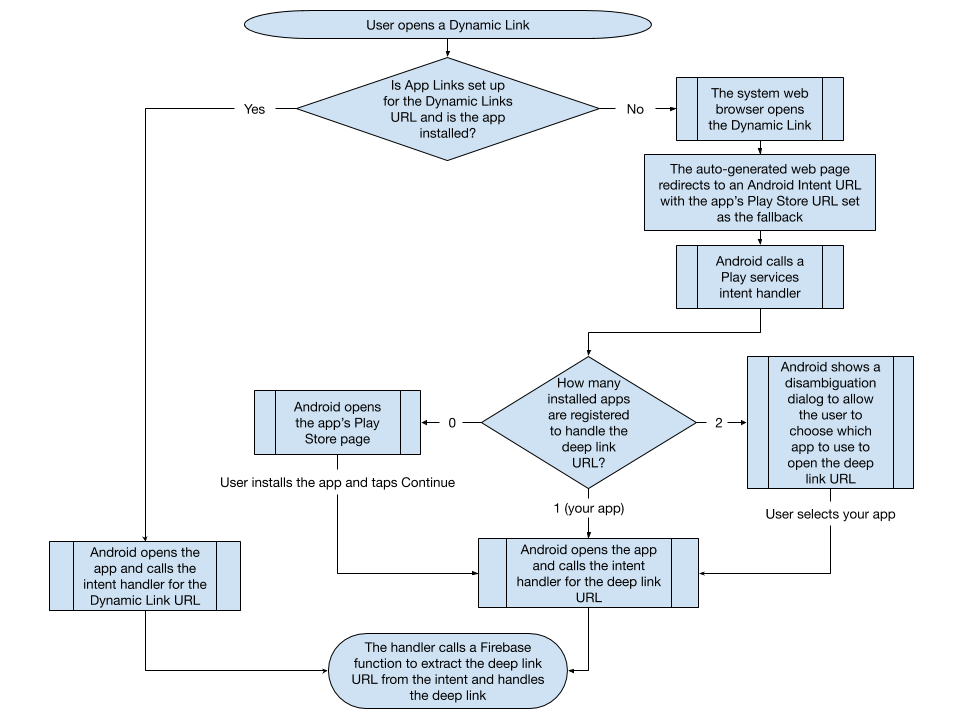
\includegraphics[width=0.83\textwidth]{images/diagramas/fdl-android-integration.png}
  \caption{Funcionamento dos dynamic links \citep{linking_firebase}}
  \label{fig:23}
\end{figure}




\newpage

\subsection{Qualidade de código}

\newpage

\section{Planificação do trabalho}\label{sec:planificacao trabalho}

De forma a obter uma visão geral do projeto e uma previsão de finalização foi realizada uma planificação 
expectável de tarefas.

\begin{figure}[htb]
    \centering
    
    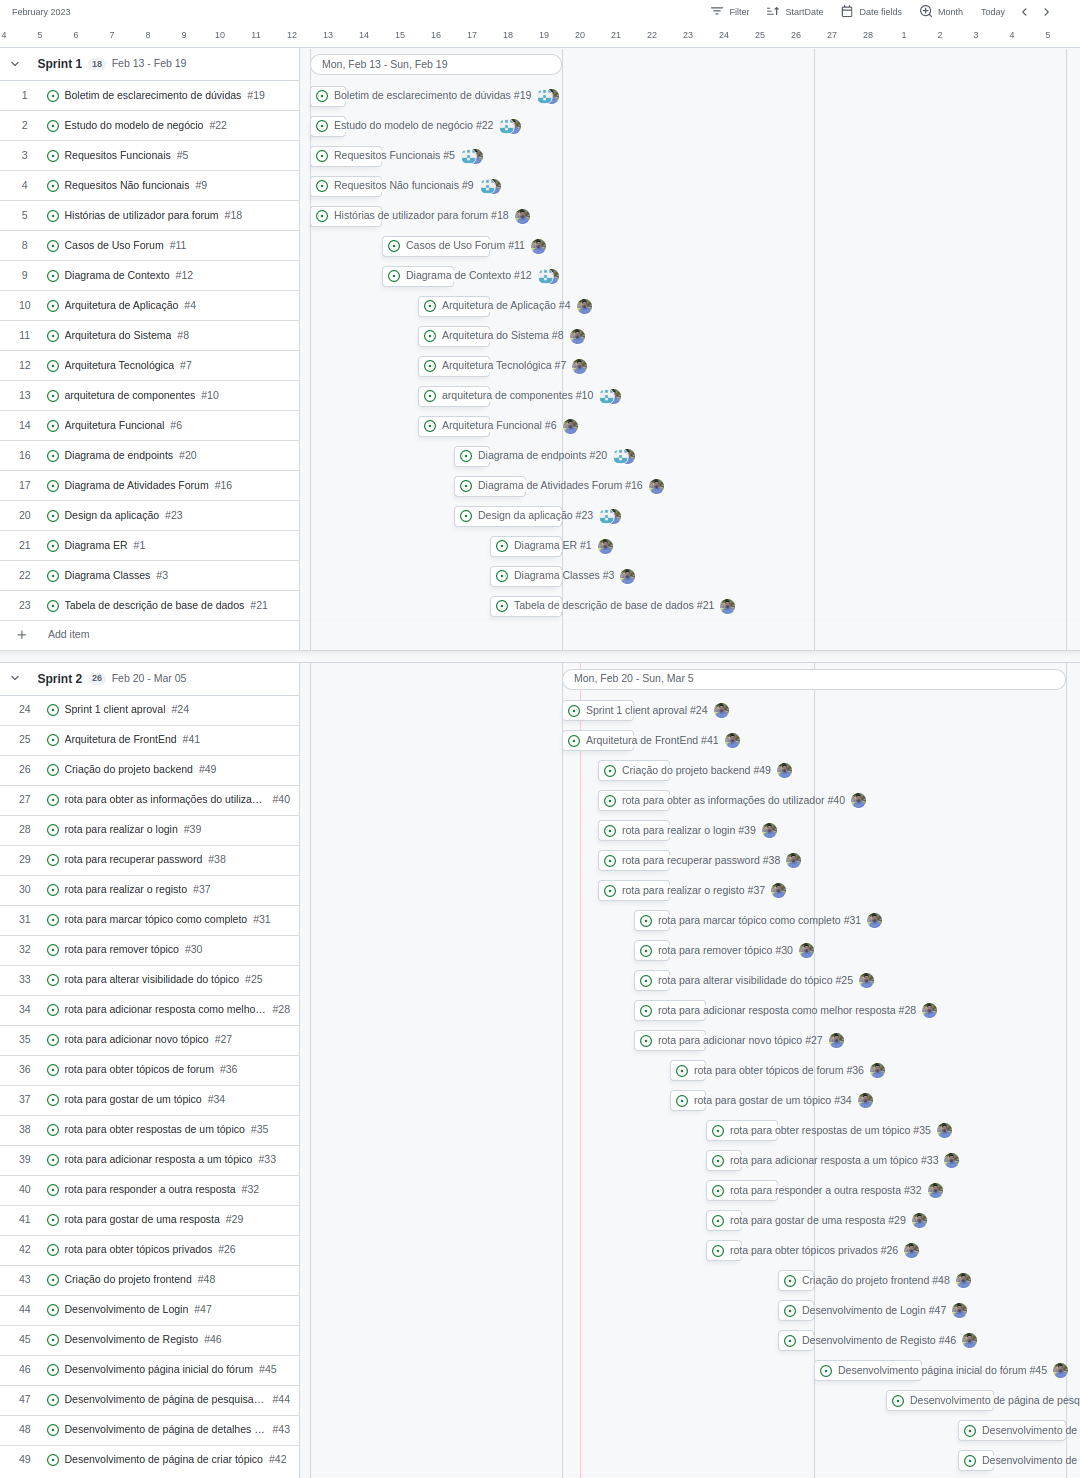
\includegraphics[width=0.75\textwidth]{images/etapa1_sprint_planning.png}
    \caption{Planeamento de sprints}
    \label{fig:1}
\end{figure}



